
% Default to the notebook output style

    


% Inherit from the specified cell style.




    
\documentclass{article}

    
    
    \usepackage{graphicx} % Used to insert images
    \usepackage{adjustbox} % Used to constrain images to a maximum size 
    \usepackage{color} % Allow colors to be defined
    \usepackage{enumerate} % Needed for markdown enumerations to work
    \usepackage{geometry} % Used to adjust the document margins
    \usepackage{amsmath} % Equations
    \usepackage{amssymb} % Equations
    \usepackage[mathletters]{ucs} % Extended unicode (utf-8) support
    \usepackage[utf8x]{inputenc} % Allow utf-8 characters in the tex document
    \usepackage{fancyvrb} % verbatim replacement that allows latex
    \usepackage{grffile} % extends the file name processing of package graphics 
                         % to support a larger range 
    % The hyperref package gives us a pdf with properly built
    % internal navigation ('pdf bookmarks' for the table of contents,
    % internal cross-reference links, web links for URLs, etc.)
    \usepackage{hyperref}
    \usepackage{longtable} % longtable support required by pandoc >1.10
    \usepackage{booktabs}  % table support for pandoc > 1.12.2
    

    
    
    \definecolor{orange}{cmyk}{0,0.4,0.8,0.2}
    \definecolor{darkorange}{rgb}{.71,0.21,0.01}
    \definecolor{darkgreen}{rgb}{.12,.54,.11}
    \definecolor{myteal}{rgb}{.26, .44, .56}
    \definecolor{gray}{gray}{0.45}
    \definecolor{lightgray}{gray}{.95}
    \definecolor{mediumgray}{gray}{.8}
    \definecolor{inputbackground}{rgb}{.95, .95, .85}
    \definecolor{outputbackground}{rgb}{.95, .95, .95}
    \definecolor{traceback}{rgb}{1, .95, .95}
    % ansi colors
    \definecolor{red}{rgb}{.6,0,0}
    \definecolor{green}{rgb}{0,.65,0}
    \definecolor{brown}{rgb}{0.6,0.6,0}
    \definecolor{blue}{rgb}{0,.145,.698}
    \definecolor{purple}{rgb}{.698,.145,.698}
    \definecolor{cyan}{rgb}{0,.698,.698}
    \definecolor{lightgray}{gray}{0.5}
    
    % bright ansi colors
    \definecolor{darkgray}{gray}{0.25}
    \definecolor{lightred}{rgb}{1.0,0.39,0.28}
    \definecolor{lightgreen}{rgb}{0.48,0.99,0.0}
    \definecolor{lightblue}{rgb}{0.53,0.81,0.92}
    \definecolor{lightpurple}{rgb}{0.87,0.63,0.87}
    \definecolor{lightcyan}{rgb}{0.5,1.0,0.83}
    
    % commands and environments needed by pandoc snippets
    % extracted from the output of `pandoc -s`
    \DefineVerbatimEnvironment{Highlighting}{Verbatim}{commandchars=\\\{\}}
    % Add ',fontsize=\small' for more characters per line
    \newenvironment{Shaded}{}{}
    \newcommand{\KeywordTok}[1]{\textcolor[rgb]{0.00,0.44,0.13}{\textbf{{#1}}}}
    \newcommand{\DataTypeTok}[1]{\textcolor[rgb]{0.56,0.13,0.00}{{#1}}}
    \newcommand{\DecValTok}[1]{\textcolor[rgb]{0.25,0.63,0.44}{{#1}}}
    \newcommand{\BaseNTok}[1]{\textcolor[rgb]{0.25,0.63,0.44}{{#1}}}
    \newcommand{\FloatTok}[1]{\textcolor[rgb]{0.25,0.63,0.44}{{#1}}}
    \newcommand{\CharTok}[1]{\textcolor[rgb]{0.25,0.44,0.63}{{#1}}}
    \newcommand{\StringTok}[1]{\textcolor[rgb]{0.25,0.44,0.63}{{#1}}}
    \newcommand{\CommentTok}[1]{\textcolor[rgb]{0.38,0.63,0.69}{\textit{{#1}}}}
    \newcommand{\OtherTok}[1]{\textcolor[rgb]{0.00,0.44,0.13}{{#1}}}
    \newcommand{\AlertTok}[1]{\textcolor[rgb]{1.00,0.00,0.00}{\textbf{{#1}}}}
    \newcommand{\FunctionTok}[1]{\textcolor[rgb]{0.02,0.16,0.49}{{#1}}}
    \newcommand{\RegionMarkerTok}[1]{{#1}}
    \newcommand{\ErrorTok}[1]{\textcolor[rgb]{1.00,0.00,0.00}{\textbf{{#1}}}}
    \newcommand{\NormalTok}[1]{{#1}}
    
    % Define a nice break command that doesn't care if a line doesn't already
    % exist.
    \def\br{\hspace*{\fill} \\* }
    % Math Jax compatability definitions
    \def\gt{>}
    \def\lt{<}
    % Document parameters
    \title{The Phase Plane Inverse Problem}
    \author{Nathan Crock}
    
    
    

    % Pygments definitions
    
\makeatletter
\def\PY@reset{\let\PY@it=\relax \let\PY@bf=\relax%
    \let\PY@ul=\relax \let\PY@tc=\relax%
    \let\PY@bc=\relax \let\PY@ff=\relax}
\def\PY@tok#1{\csname PY@tok@#1\endcsname}
\def\PY@toks#1+{\ifx\relax#1\empty\else%
    \PY@tok{#1}\expandafter\PY@toks\fi}
\def\PY@do#1{\PY@bc{\PY@tc{\PY@ul{%
    \PY@it{\PY@bf{\PY@ff{#1}}}}}}}
\def\PY#1#2{\PY@reset\PY@toks#1+\relax+\PY@do{#2}}

\expandafter\def\csname PY@tok@gd\endcsname{\def\PY@tc##1{\textcolor[rgb]{0.63,0.00,0.00}{##1}}}
\expandafter\def\csname PY@tok@gu\endcsname{\let\PY@bf=\textbf\def\PY@tc##1{\textcolor[rgb]{0.50,0.00,0.50}{##1}}}
\expandafter\def\csname PY@tok@gt\endcsname{\def\PY@tc##1{\textcolor[rgb]{0.00,0.27,0.87}{##1}}}
\expandafter\def\csname PY@tok@gs\endcsname{\let\PY@bf=\textbf}
\expandafter\def\csname PY@tok@gr\endcsname{\def\PY@tc##1{\textcolor[rgb]{1.00,0.00,0.00}{##1}}}
\expandafter\def\csname PY@tok@cm\endcsname{\let\PY@it=\textit\def\PY@tc##1{\textcolor[rgb]{0.25,0.50,0.50}{##1}}}
\expandafter\def\csname PY@tok@vg\endcsname{\def\PY@tc##1{\textcolor[rgb]{0.10,0.09,0.49}{##1}}}
\expandafter\def\csname PY@tok@m\endcsname{\def\PY@tc##1{\textcolor[rgb]{0.40,0.40,0.40}{##1}}}
\expandafter\def\csname PY@tok@mh\endcsname{\def\PY@tc##1{\textcolor[rgb]{0.40,0.40,0.40}{##1}}}
\expandafter\def\csname PY@tok@go\endcsname{\def\PY@tc##1{\textcolor[rgb]{0.53,0.53,0.53}{##1}}}
\expandafter\def\csname PY@tok@ge\endcsname{\let\PY@it=\textit}
\expandafter\def\csname PY@tok@vc\endcsname{\def\PY@tc##1{\textcolor[rgb]{0.10,0.09,0.49}{##1}}}
\expandafter\def\csname PY@tok@il\endcsname{\def\PY@tc##1{\textcolor[rgb]{0.40,0.40,0.40}{##1}}}
\expandafter\def\csname PY@tok@cs\endcsname{\let\PY@it=\textit\def\PY@tc##1{\textcolor[rgb]{0.25,0.50,0.50}{##1}}}
\expandafter\def\csname PY@tok@cp\endcsname{\def\PY@tc##1{\textcolor[rgb]{0.74,0.48,0.00}{##1}}}
\expandafter\def\csname PY@tok@gi\endcsname{\def\PY@tc##1{\textcolor[rgb]{0.00,0.63,0.00}{##1}}}
\expandafter\def\csname PY@tok@gh\endcsname{\let\PY@bf=\textbf\def\PY@tc##1{\textcolor[rgb]{0.00,0.00,0.50}{##1}}}
\expandafter\def\csname PY@tok@ni\endcsname{\let\PY@bf=\textbf\def\PY@tc##1{\textcolor[rgb]{0.60,0.60,0.60}{##1}}}
\expandafter\def\csname PY@tok@nl\endcsname{\def\PY@tc##1{\textcolor[rgb]{0.63,0.63,0.00}{##1}}}
\expandafter\def\csname PY@tok@nn\endcsname{\let\PY@bf=\textbf\def\PY@tc##1{\textcolor[rgb]{0.00,0.00,1.00}{##1}}}
\expandafter\def\csname PY@tok@no\endcsname{\def\PY@tc##1{\textcolor[rgb]{0.53,0.00,0.00}{##1}}}
\expandafter\def\csname PY@tok@na\endcsname{\def\PY@tc##1{\textcolor[rgb]{0.49,0.56,0.16}{##1}}}
\expandafter\def\csname PY@tok@nb\endcsname{\def\PY@tc##1{\textcolor[rgb]{0.00,0.50,0.00}{##1}}}
\expandafter\def\csname PY@tok@nc\endcsname{\let\PY@bf=\textbf\def\PY@tc##1{\textcolor[rgb]{0.00,0.00,1.00}{##1}}}
\expandafter\def\csname PY@tok@nd\endcsname{\def\PY@tc##1{\textcolor[rgb]{0.67,0.13,1.00}{##1}}}
\expandafter\def\csname PY@tok@ne\endcsname{\let\PY@bf=\textbf\def\PY@tc##1{\textcolor[rgb]{0.82,0.25,0.23}{##1}}}
\expandafter\def\csname PY@tok@nf\endcsname{\def\PY@tc##1{\textcolor[rgb]{0.00,0.00,1.00}{##1}}}
\expandafter\def\csname PY@tok@si\endcsname{\let\PY@bf=\textbf\def\PY@tc##1{\textcolor[rgb]{0.73,0.40,0.53}{##1}}}
\expandafter\def\csname PY@tok@s2\endcsname{\def\PY@tc##1{\textcolor[rgb]{0.73,0.13,0.13}{##1}}}
\expandafter\def\csname PY@tok@vi\endcsname{\def\PY@tc##1{\textcolor[rgb]{0.10,0.09,0.49}{##1}}}
\expandafter\def\csname PY@tok@nt\endcsname{\let\PY@bf=\textbf\def\PY@tc##1{\textcolor[rgb]{0.00,0.50,0.00}{##1}}}
\expandafter\def\csname PY@tok@nv\endcsname{\def\PY@tc##1{\textcolor[rgb]{0.10,0.09,0.49}{##1}}}
\expandafter\def\csname PY@tok@s1\endcsname{\def\PY@tc##1{\textcolor[rgb]{0.73,0.13,0.13}{##1}}}
\expandafter\def\csname PY@tok@sh\endcsname{\def\PY@tc##1{\textcolor[rgb]{0.73,0.13,0.13}{##1}}}
\expandafter\def\csname PY@tok@sc\endcsname{\def\PY@tc##1{\textcolor[rgb]{0.73,0.13,0.13}{##1}}}
\expandafter\def\csname PY@tok@sx\endcsname{\def\PY@tc##1{\textcolor[rgb]{0.00,0.50,0.00}{##1}}}
\expandafter\def\csname PY@tok@bp\endcsname{\def\PY@tc##1{\textcolor[rgb]{0.00,0.50,0.00}{##1}}}
\expandafter\def\csname PY@tok@c1\endcsname{\let\PY@it=\textit\def\PY@tc##1{\textcolor[rgb]{0.25,0.50,0.50}{##1}}}
\expandafter\def\csname PY@tok@kc\endcsname{\let\PY@bf=\textbf\def\PY@tc##1{\textcolor[rgb]{0.00,0.50,0.00}{##1}}}
\expandafter\def\csname PY@tok@c\endcsname{\let\PY@it=\textit\def\PY@tc##1{\textcolor[rgb]{0.25,0.50,0.50}{##1}}}
\expandafter\def\csname PY@tok@mf\endcsname{\def\PY@tc##1{\textcolor[rgb]{0.40,0.40,0.40}{##1}}}
\expandafter\def\csname PY@tok@err\endcsname{\def\PY@bc##1{\setlength{\fboxsep}{0pt}\fcolorbox[rgb]{1.00,0.00,0.00}{1,1,1}{\strut ##1}}}
\expandafter\def\csname PY@tok@kd\endcsname{\let\PY@bf=\textbf\def\PY@tc##1{\textcolor[rgb]{0.00,0.50,0.00}{##1}}}
\expandafter\def\csname PY@tok@ss\endcsname{\def\PY@tc##1{\textcolor[rgb]{0.10,0.09,0.49}{##1}}}
\expandafter\def\csname PY@tok@sr\endcsname{\def\PY@tc##1{\textcolor[rgb]{0.73,0.40,0.53}{##1}}}
\expandafter\def\csname PY@tok@mo\endcsname{\def\PY@tc##1{\textcolor[rgb]{0.40,0.40,0.40}{##1}}}
\expandafter\def\csname PY@tok@kn\endcsname{\let\PY@bf=\textbf\def\PY@tc##1{\textcolor[rgb]{0.00,0.50,0.00}{##1}}}
\expandafter\def\csname PY@tok@mi\endcsname{\def\PY@tc##1{\textcolor[rgb]{0.40,0.40,0.40}{##1}}}
\expandafter\def\csname PY@tok@gp\endcsname{\let\PY@bf=\textbf\def\PY@tc##1{\textcolor[rgb]{0.00,0.00,0.50}{##1}}}
\expandafter\def\csname PY@tok@o\endcsname{\def\PY@tc##1{\textcolor[rgb]{0.40,0.40,0.40}{##1}}}
\expandafter\def\csname PY@tok@kr\endcsname{\let\PY@bf=\textbf\def\PY@tc##1{\textcolor[rgb]{0.00,0.50,0.00}{##1}}}
\expandafter\def\csname PY@tok@s\endcsname{\def\PY@tc##1{\textcolor[rgb]{0.73,0.13,0.13}{##1}}}
\expandafter\def\csname PY@tok@kp\endcsname{\def\PY@tc##1{\textcolor[rgb]{0.00,0.50,0.00}{##1}}}
\expandafter\def\csname PY@tok@w\endcsname{\def\PY@tc##1{\textcolor[rgb]{0.73,0.73,0.73}{##1}}}
\expandafter\def\csname PY@tok@kt\endcsname{\def\PY@tc##1{\textcolor[rgb]{0.69,0.00,0.25}{##1}}}
\expandafter\def\csname PY@tok@ow\endcsname{\let\PY@bf=\textbf\def\PY@tc##1{\textcolor[rgb]{0.67,0.13,1.00}{##1}}}
\expandafter\def\csname PY@tok@sb\endcsname{\def\PY@tc##1{\textcolor[rgb]{0.73,0.13,0.13}{##1}}}
\expandafter\def\csname PY@tok@k\endcsname{\let\PY@bf=\textbf\def\PY@tc##1{\textcolor[rgb]{0.00,0.50,0.00}{##1}}}
\expandafter\def\csname PY@tok@se\endcsname{\let\PY@bf=\textbf\def\PY@tc##1{\textcolor[rgb]{0.73,0.40,0.13}{##1}}}
\expandafter\def\csname PY@tok@sd\endcsname{\let\PY@it=\textit\def\PY@tc##1{\textcolor[rgb]{0.73,0.13,0.13}{##1}}}

\def\PYZbs{\char`\\}
\def\PYZus{\char`\_}
\def\PYZob{\char`\{}
\def\PYZcb{\char`\}}
\def\PYZca{\char`\^}
\def\PYZam{\char`\&}
\def\PYZlt{\char`\<}
\def\PYZgt{\char`\>}
\def\PYZsh{\char`\#}
\def\PYZpc{\char`\%}
\def\PYZdl{\char`\$}
\def\PYZhy{\char`\-}
\def\PYZsq{\char`\'}
\def\PYZdq{\char`\"}
\def\PYZti{\char`\~}
% for compatibility with earlier versions
\def\PYZat{@}
\def\PYZlb{[}
\def\PYZrb{]}
\makeatother


    % Exact colors from NB
    \definecolor{incolor}{rgb}{0.0, 0.0, 0.5}
    \definecolor{outcolor}{rgb}{0.545, 0.0, 0.0}



    
    % Prevent overflowing lines due to hard-to-break entities
    \sloppy 
    % Setup hyperref package
    \hypersetup{
      breaklinks=true,  % so long urls are correctly broken across lines
      colorlinks=true,
      urlcolor=blue,
      linkcolor=darkorange,
      citecolor=darkgreen,
      }
    % Slightly bigger margins than the latex defaults
    
    \geometry{verbose,tmargin=1in,bmargin=1in,lmargin=1in,rmargin=1in}
    
    

    \begin{document}
    
    
    \maketitle
    
    

    
\section{Objective}\label{sec:objective}

\textbf{Given a set of equilibria and their stability, construct a
system of equations that produces "similar" dynamics to those determined
by the equilibria.} \\

\section{Introduction}\label{sec:introduction}

We will attempt to address this in two dimensions. Take a general planar system of the following form.

\begin{align*}
\dot x &= f(x,y) \\
\dot y &= g(x,y)
\end{align*}

\noindent What form should $f(x,y)$ and $g(x,y)$ take? We will first show that
any single equilibrium in two dimensions can be reproduced by a coupled system
of polynomials.

\begin{align}
    \begin{split}
    f(x,y) &= \text{P}_1(x)+y \\
    g(x,y) &= -x+\text{P}_2(y) \label{eq:system}
    \end{split}
\end{align}

\noindent where P$_1(x)$ and P$_2(y)$ are arbitrary polynomials of degree greater than 1.
This form was chosen so that the nullclines could be explicitly defined
and would be conducive to analysis. The nullclines are given by

\begin{align}
    y &= -\text{P}_1(x) \label{eq:x-null}\\ 
    x &= \text{P}_2(y) \label{eq:y-null}
\end{align}

\noindent and the Jacobian of the system is given by

\begin{equation}
J(x,y) = \begin{bmatrix}
       p_1 & 1 \\
       -1 & p_2
\end{bmatrix} \label{eq:jacobian}
 \end{equation}

\noindent where for notational brevity we are referring to the derivatives as
$\frac{d\text{P}_1}{dx}(x) \equiv p_1$ and $\frac{d\text{P}_2}{dy}(y) \equiv p_2$.
We can quickly see the trace and determinant.

\begin{align}
    \text{Trace}(J) &= \tau(p_1,p_2) = p_1 + p_2 \label{eq:trace} \\ 
    \text{Det}(J) &= \Delta(p_1,p_2) = p_1 p_2 +1 \label{eq:det}
\end{align}

\noindent The eigenvalues of the Jacobian determine the type and stability of
nonhyperbolic equilibria. The characteristic for this system is given by

\begin{equation*}
    \begin{vmatrix}
        p_1-\lambda & 1 \\
        -1 & p_2-\lambda
    \end{vmatrix} = (p_1-\lambda)(p_2-\lambda)+1 
\end{equation*}

\begin{equation*}
    \Rightarrow \lambda^2 - (p_1+p_2)\lambda + p_1 p_2 +1
\end{equation*}

\begin{equation}
    \Rightarrow \lambda^2-\tau \lambda+\Delta \label{eq:characteristic}
\end{equation}

\noindent and given the characteristic we find the eigenvalues.

\[\lambda = \frac{\tau \pm \sqrt{\tau^2-4\Delta}}{2}\]

\noindent In conventional dynamics theory the type of equilibria for $\Delta>0$ is determined by
the sign of the radicand $\tau^2-4\Delta$ and their stability is
determined by the sign of $\tau$ and $\Delta$. This relationship is usually
depicted in a $\tau$ vs $\Delta$ plot such as the one shown below in figure
\ref{fig:tauvsdelta}.

\begin{figure}[h]
\centering
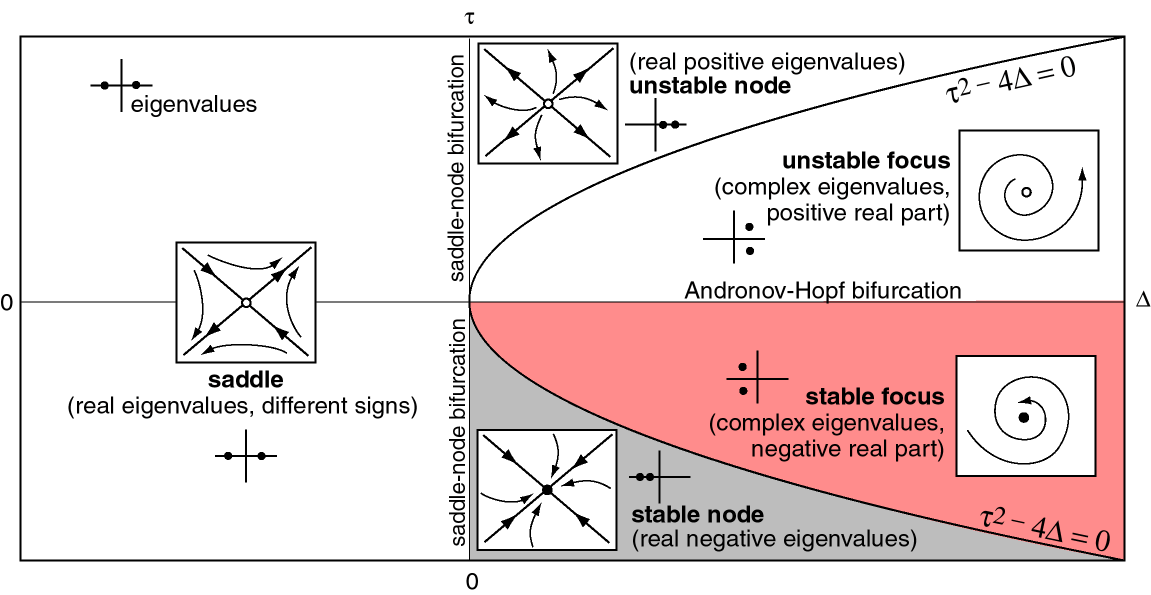
\includegraphics[scale=0.37]{figures/tauvsdelta.png}
\caption{Source: http://www.intechopen.com/source/html/40762/media/image13.png}
\label{fig:tauvsdelta}
\end{figure}

In general $\tau$ and $\Delta$ can take on all values and collectively
describe all hyperbolic equilibria in two dimensions. Given that $\text{P}_1(x)$ and
$\text{P}_2(y)$ are polynomials we know that their derivatives can take on any
value $p_1,p_2 \hspace{3pt} \in \hspace{3pt} (-\infty,\infty)$. Also,
because our general system above produces continuous $\tau$ and
$\Delta$ as seen in equations ~\ref{eq:trace} and ~\ref{eq:det}  we see that it is capable of reproducing all equilibria in two
dimensions. Or in simpler terms, we know that two linear polynomials are sufficient to
produce any equilibria and the form presented in this document reduces to a
linear system, therefore the system ~\ref{eq:system} can also produce any
equilibria in the plane. \\

To make this more concrete let us look at a $p_1$ vs. $p_2$ plot to examine the relationships which
produce the various types of equilibria. There are three things we will use, the
trace and determinant, equations ~\ref{eq:trace} and ~\ref{eq:det}, and the radicand shown below.

\begin{equation}
    \tau^2-4\Delta \label{eq:radicand}
\end{equation}

\noindent The idea is to express each in terms of $p_1$, $p_2$ and then
examine the collection of inequalities, much like in figure ~\ref{fig:tauvsdelta}. We start by looking at the trace, $\tau$.

\begin{gather}
    \tau(p_1,p_2) = p_1+p_2 = 0 \nonumber \\
    p_1 = -p_2 \label{eq:zerotrace}
\end{gather}

\noindent We know that the trace determines stability. If the trace is 
positive, the equilibrium is unstable. If the trace is negative, the equilibrium
is stable. Therefore equation ~\ref{eq:zerotrace} will represent the partition
between stablility and instability. Any point along the line produces a
neutrally stable center point which is where a Hopf bifurcation occurs. \\

\noindent Next we look at the determinant. 

\begin{gather}
    \Delta(p_1,p_2) = p_1p_2+1 = 0 \nonumber \\
    p_1=-\frac{1}{p_2} \label{eq:zerodet}
\end{gather}

\noindent We know that when the determinant is negative, we have a saddle
node. Therefore equation ~\ref{eq:zerodet} will represent the partition between
saddle nodes and all other equilibria. All points along the curve are where
nodes and saddles fuse or split, also known as a Saddle Node bifurcation. \\


\noindent Lastly, we look at the radicand. Like before we will use equations
~\ref{eq:trace} and ~\ref{eq:det} to express the radicand in terms of $p_1$ and
$p_2$.

\begin{align}
    \tau^2(p_1,p_2) - 4\Delta(p_1,p_2) &=0 \nonumber \\
    (p_1+p_2)^2-4(p_1p_2+1) &=0 \nonumber \\
    p_1^2+2p_1p_2+p_2^2-4p_1p_2-4 &=0 \nonumber \\
    p_1^2-2p_1p_2+p_2^2-4 &=0 \nonumber \\
    (p_1-p_2)^2-4 &=0 \nonumber \\
    (p_1-p_2-2)(p_1-p_2+2) &=0 \nonumber \\
    p_1 = p_2 \pm 2 \label{eq:zeroradicand}
\end{align}

\noindent The sign of the radicand determines the type of equilibria. If the
radicand is positive we have real eigenvalues and the equilibrium is a node. If
the radicand is negative we have imaginary eigenvalues and the equilibrium is a
spiral. Therefore the two lines in equation ~\ref{eq:zeroradicand} are the
partitions between nodes and spirals. In other words $|p_1-p_2| < 2$ are
the parameters that create a spiral and $|p_1-p_2| > 2$ are the parameters that
create a node. Well it is only a node if $p_1p_2 >-1$ is also satisfied, i.e. it
is not a saddle node. All
$p_1$ and $p_2$ satisfying $|p_1-p_2|=0$ create degenerate nodes, or stars. The
plot of $p_1$ vs $p_2$ is shown in figure ~\ref{fig:p1vsp2}.\\

\begin{figure}[h!]
\centering
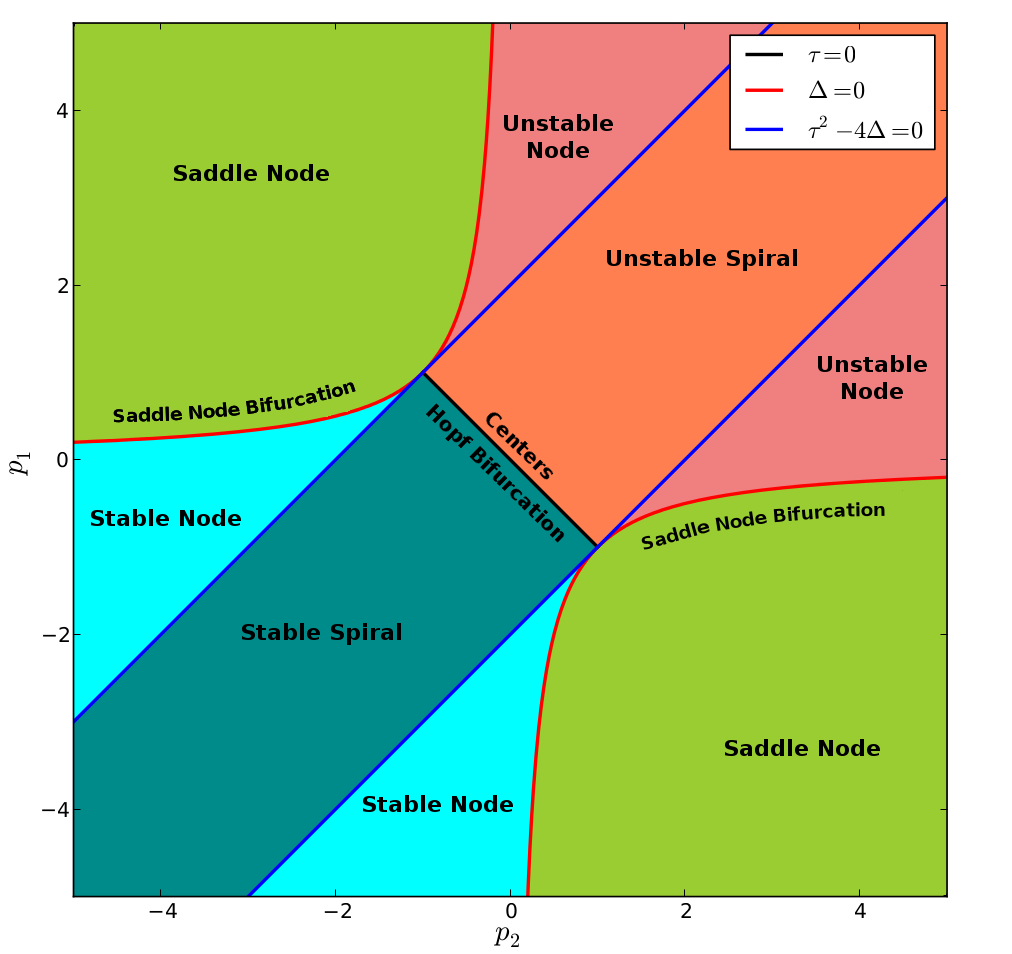
\includegraphics[scale=0.70]{figures/p1vsp2_full_labels.png}
\caption{We plot the three partitions in equations ~\ref{eq:zerotrace},
    ~\ref{eq:zerodet}, ~\ref{eq:zeroradicand} and label the different regions of
    the parameter space with their associated equilibria types and stability.
The black line in the middle is $\tau=0$. As this is where the trace transitions
from negative to positive, it divides the plot into stable and unstable regions.
The red line is where $\Delta=0$. This divides the region between saddle nodes,
and everything else. Lastly, the blue lines are where $\tau^2-4\Delta=0$. They
divide the regions between where nodes and spirals occur.}
\label{fig:p1vsp2}
\end{figure}

\section{Angle Dependent Dynamics}\label{sec:angles}

Using implicit differentiation we can find the slope of each nullcline in phase
space ($y$ vs. $x$) as

\begin{align}
-\frac{f_x}{f_y} &= -p_1 \\
-\frac{g_x}{g_y} &= \frac{1}{p_2}
\end{align}

\noindent In the $y$ vs $x$ phase space we'll define a vector tangent to each
nullcline as

\begin{align}
\vec{T_x} &= 1\hat{i} + -p_1\hat{j} \\
\vec{T_y} &= p_2\hat{i} + 1\hat{j} 
\end{align}

We are interested in the angle between these vectors at an equilibria,
therefore we will use the following formula\ldots{}

\[\theta = \cos^{-1}(\frac{\vec{T_x}\cdot \vec{T_y}}{\|T_x\| \|T_y\|})\]

Starting with the numerator we get\ldots{}

\[\vec{T_x}\cdot \vec{T_y} = p_2-p_1\]

And in the denominator

\[\|T_x\| \|T_y\| = \sqrt{1+p^2_1}\sqrt{1+p^2_2}\]

The objective here is to find the angle between the tangent vectors in
terms of the eigenvalues of the system. We will need to convert the
numerator and denominator into expressions of only eigenvalues. For this
we will be using the handy fact from linear algebra that the trace of a
matrix is equal to the sum of its eigenvalues,
$\tau=\lambda_1+\lambda_2$, and the determinant of a matrix is equal to
the product of its eigenvalues, $\Delta = \lambda_1 \lambda_2$. \\

\textbf{TO DO: elegant algebra leading to the following formulas (don't
have time now)} \\

Thus we find the angle between the tangent vectors at the equilibria is
given by

\[\theta(\lambda_1,\lambda_2) = \cos^{-1}\Bigg (\pm \sqrt{\frac{(\lambda_1-\lambda_2)^2+4}{(\lambda_1+\lambda_2)^2+(\lambda_1 \lambda_2-2)^2}}\Bigg )\]

Or, in terms of the trace and determinant

\[\theta(\lambda_1,\lambda_2) = \cos^{-1}\Bigg (\pm \sqrt{\frac{\tau^2+4(1-\Delta)}{\tau^2+(\Delta-2)^2}}\Bigg )\]

We will show that this is defined for all nonzero $\lambda_1$ and
$\lambda_2$. We needn't worry about the degenerate case as the
Hartman-Grobman theory tells us the Jacobian is not guaranteed to
correctly determine the stability of non-hyperbolic equilibria. We need
to show three things.

\begin{enumerate}
\def\labelenumi{\arabic{enumi}.}
\itemsep1pt\parskip0pt\parsep0pt
\item
  The denominator is never zero
\item
  The radicand is always positive
\item
  The magnitude of the argument to $\cos^{-1}$ is bounded by one
\end{enumerate}

The second equation is found by algebraic manipulations and subsitutions
of the first. Therefore showing any of the properties for one equation
implies it is true for the other. \\

\begin{enumerate}
\def\labelenumi{\arabic{enumi}.}
\itemsep1pt\parskip0pt\parsep0pt
\item
    \emph{The denominator is never zero} \\
  By inspection we see that both terms in the denominator are
  squared (in both equations). Thus, the denominator is nonzero for
  nonzero eigenvalues. \\
\item
    \emph{The radicand is always positive} \\
By inspecting the first equation we see that all terms in
the radicand are positive, and we are done. \\
\item
    \emph{The magnitude of the argument to $\cos^{-1}$ is bounded by one} \\
Looking at the second equation\ldots{} \\

\[\frac{\tau^2+4(1-\Delta)}{\tau^2+(\Delta-2)^2} < 1 \hspace{10pt} \rightarrow \hspace{10pt} \tau^2+4(1-\Delta) < \tau^2+(\Delta-2)^2\]

Recalling that the denominator is nonzero we do not flip the inequality.
We expand both sides,

\[\tau^2-4\Delta+4 < \tau^2+\Delta^2-4\Delta+4 \hspace{10pt} \rightarrow \hspace{4pt} 0 < \Delta^2\]

which is always true for nonzero eigenvalues. \\

\end{enumerate}

\textbf{TO DO: Demonstrate with some small examples} \\

    % Add a bibliography block to the postdoc
    
    
    
\end{document}
